\section{Propagation of particles in ice}
\label{sec:particle-interactions}
Neutrinos interacting with the ice mostly interact via Deep Inelastic Scattering (DIS), creating muons, electromagnetic showers, and hadronic showers, depending on the flavor of the neutrino and interaction type.
The secondary particles produced by those interactions travel through the ice at highly relativistic velocities and lose energy primarily through ionization, bremsstrahlung, pair production and photo-nuclear interactions. The fraction that each of these mechanisms contributes to the total energy loss of the particle depends on the type of particle and its energy. When they are electrically charged, they also give off Cherenkov radiation that is then measured by IceCube.

\subsection{Cherenkov Effect}

The IceCube Neutrino Observatory relies entirely on the Cherenkov effect to detect particle interactions. It is created by any electrically charged particle travelling through a transparent medium with velocities faster than the speed of light in that medium, $c/n$, where $n$ is the refractive index of the medium. This produces a cone of light moving with the particle similar to a super-sonic shock that is generated by an object travelling through a gas at a velocity above the speed of sound. The effect can be most easily understood according to Huygen's principle as a superposition of spherical light emissions that are produced every time that the particle displaces the charges in the dielectric medium in its closest vicinity, as shown in Figure~\ref{fig:cherenkov-sketch}. When the particle is over-taking its own light emissions, they overlap coherently and form a conical light front as illustrated in the bottom panel of Figure~\ref{fig:cherenkov-sketch}.
\begin{marginfigure}
    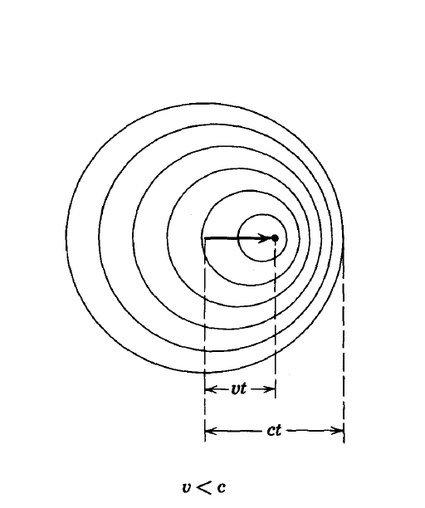
\includegraphics[width=\textwidth]{figures/icecube/cherenkov/cherenkov_slow.jpeg}
    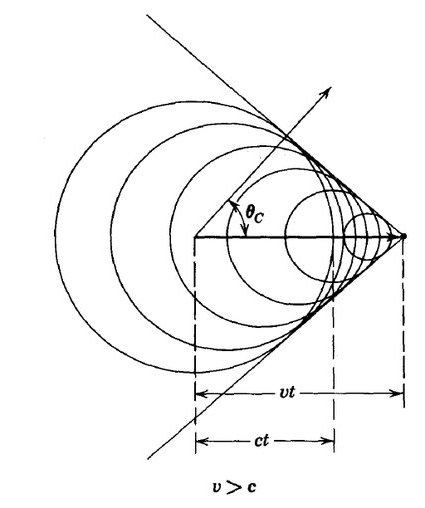
\includegraphics[width=\textwidth]{figures/icecube/cherenkov/cherenkov_fast.jpeg}
    \caption{An electrically charged particle emitting light while travelling below (upper panel) and above (lower panel) the speed of light in a medium. Image taken from \cite{jackson2012classical}.}
    \label{fig:cherenkov-sketch}
\end{marginfigure}
When the velocity of the particle is very close to the speed of light, as is the case for all (known) particles observable by IceCube, the opening angle of the cone only depends on the refractive index of the medium with
\begin{equation}
    \cos(\vartheta_c)=\frac{1}{\beta n}\;,
\end{equation}
where $n$ is the index of refraction and $\vartheta_c$ is the Cherenkov opening angle.

The frequency spectrum of the Cherenkov emissions of highly relativistic particles depends only on the charge of the particle, $q$, and the (wavelength-dependent) index of refraction, $n(\omega)$, and permeability, $\mu(\omega)$, of the medium. The emitted energy per unit of distance and frequency is given by the Frank-Tamm-Equation, which simplifies in the case of $v\approx c$ to
\begin{equation}
    \frac{\drm E}{\drm x \drm \omega}=\frac{q^2}{4\pi}\mu(\omega)\omega\left(1-\frac{1}{n^2(\omega)}\right)\,.
\end{equation}
The equation shows that the intensity of the Cherenkov emission generally increases with frequency, and indeed the strongest emissions are in the ultraviolet part of the spectrum.

\subsection{Muons}
\label{sec:muon-propagation}
At energies below 100~GeV, the dominant energy loss for muons is via ionization, and has only a weak dependence on energy. Because the ionization loss is continuous and nearly constant, muons at these energies produce long, track-like signatures in the detector. Above 100~GeV, the losses due to bremsstrahlung, pair production and photo-nuclear interactinos rise quickly in their amplitude and become dominant over ionization at $\sim$1~TeV. The total average energy loss per unit distance, $\left<\drm E/\drm x\right>$, can be approximated combining all radiative energy losses (i.e. all losses except for ionization) into one component and adding it to the ionization loss such that
\begin{equation}
    \left<-\frac{\drm E}{\drm x}\right> = a_I(E) + b_R(E)E\,,
\end{equation}
where $a_I(E)$ and $b_R(E)$ are slowly changing functions describing the ionization loss and the radiative losses, respectively\cite{muonstoppingpower}. For the energy ranges relevant for this work, the energy dependence of $a_I(E)$ and $b_R(E)$ is weak enough such that they can be approximated as constant numbers with $a_I(E)\approx 2\;\mathrm{MeV/cm}$ and $b_R(E)\approx3.4\times10^{-6}\;\mathrm{cm^{-1}}$\cite{muonstoppingpower}. In this approximation, we can calculate the average length of a muon track, $\left<L\right>$, as a function of energy with
\begin{equation}
    \left<L\right>=\frac{1}{b_R}\log\left(\frac{b_R}{a_I}E + 1\right)\,,
\end{equation}
which gives an average travel distance of 50~m at 10~GeV and 460~m at 100~GeV.

\subsection{Electromagnetic Showers}
\label{sec:em-showers}
In contrast to muons, electrons and positrons lose their energy very quickly by emitting very highly energetic photons due to bremsstrahlung. The energy of the emitted photons is high enough that they spontaneously produce pairs of electrons and positrons. This process is repeated until the electrons and positrons reach their critical energy, which is approximately 78~MeV in water ice\sidecite{pdg}. Below the critical energy, ionization takes over as the predominant mechanism of energy loss, which produces no new shower particles. Another important quantity is the \emph{radiation length}, $X_0$, defined as the distance at which the energy of an electron is reduced to $\nicefrac{1}{e}$ of its initial energy via bremsstrahlung, which is 36~cm in ice\cite{pdg}. The radiation length also determines the scale of the longitudinal development of the shower. Expressing distances in units of radiation length as $t=x/X_0$, the shower intensity follows roughly a gamma distribution parametrized as
\begin{equation}
    \frac{\drm E}{\drm t} = E_0 b \frac{(bt)^{a-1}e^{-bt}}{\Gamma(a)}\;,
\end{equation}
where the parameters $a$ and $b$ need to be fit empirically\cite{pdg}. Their values for electrons, positrons and photons interacting in ice have been determined from GEANT4\sidecite{geant4} shower simulations in\sidecite{RADEL2013102} to be
\begin{align}
    a &\approx 2.01 + 1.46 \log_{10}(E_0/\mathrm{GeV}),\; b\approx 0.63\; & (e^+,e^-), \\
    a &\approx 2.84 + 1.34 \log_{10}(E_0/\mathrm{GeV}),\; b\approx 0.65\; & (\gamma).\label{eq:shower-params}
\end{align}
The shower reaches its maximum intensity at a distance of
\begin{equation}
    t_{\mathrm{max}}=\frac{a-1}{b}\;,
\end{equation}
which corresponds to a logarithmic growth of the size of the cascade according to eq.~\ref{eq:shower-params}. The electrically charged components of the electromagnetic shower produce Cherenkov light, where the emissions peak at the Cherenkov angle since the secondary particles are emitted very close to the forward direction as shown in figure~\ref{fig:cherenkov_angular_profile_cascade}.

\begin{marginfigure}
    \centering
    \tikzsetnextfilename{cascade_cherenkov_angular_dist}%
    % This file was created with tikzplotlib v0.10.1.
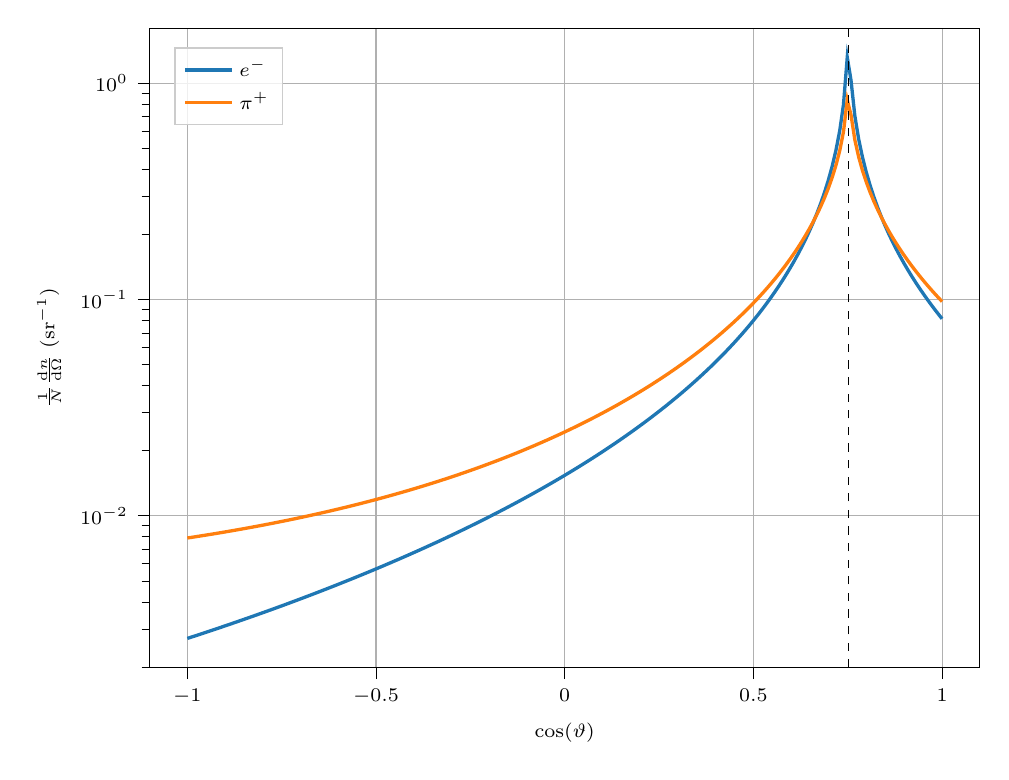
\begin{tikzpicture}

\definecolor{darkgray176}{RGB}{176,176,176}
\definecolor{darkorange25512714}{RGB}{255,127,14}
\definecolor{lightgray204}{RGB}{204,204,204}
\definecolor{steelblue31119180}{RGB}{31,119,180}

\begin{axis}[
height=0.8\linewidth,
legend cell align={left},
legend style={
  fill opacity=0.8,
  draw opacity=1,
  text opacity=1,
  at={(0.03,0.97)},
  anchor=north west,
  draw=lightgray204
},
log basis y={10},
minor xtick={},
minor ytick={0.0002,0.0003,0.0004,0.0005,0.0006,0.0007,0.0008,0.0009,0.002,0.003,0.004,0.005,0.006,0.007,0.008,0.009,0.02,0.03,0.04,0.05,0.06,0.07,0.08,0.09,0.2,0.3,0.4,0.5,0.6,0.7,0.8,0.9,2,3,4,5,6,7,8,9,20,30,40,50,60,70,80,90,200,300,400,500,600,700,800,900},
tick align=outside,
tick pos=left,
width=\linewidth,
x grid style={darkgray176},
xlabel={\(\scriptstyle \cos(\vartheta)\)},
xmajorgrids,
xmin=-1.1, xmax=1.1,
xtick style={color=black},
xtick={-1.5,-1,-0.5,0,0.5,1,1.5},
xticklabels={
\(\scriptstyle -1.5\),
\(\scriptstyle -1\),
\(\scriptstyle -0.5\),
\(\scriptstyle 0\),
\(\scriptstyle 0.5\),
\(\scriptstyle 1\),
\(\scriptstyle 1.5\)
},
y grid style={darkgray176},
ylabel={\(\scriptstyle \frac{1}{N}\frac{\mathrm{d}n}{\mathrm{d}\Omega}\;(\mathrm{sr^{-1}})\)},
ymajorgrids,
ymin=0.00198893054244642, ymax=1.79304902414132,
ymode=log,
ytick style={color=black},
ytick={0.0001,0.001,0.01,0.1,1,10,100},
yticklabels={
  \(\scriptstyle {10^{-4}}\),
  \(\scriptstyle {10^{-3}}\),
  \(\scriptstyle {10^{-2}}\),
  \(\scriptstyle {10^{-1}}\),
  \(\scriptstyle {10^{0}}\),
  \(\scriptstyle {10^{1}}\),
  \(\scriptstyle {10^{2}}\)
}
]
% \addlegendimage{empty legend}
% \addlegendentry{\hspace{-.6cm}\(\scriptstyle Primary particle\)}
\addplot [very thick, steelblue31119180]
table {%
-1 0.00270979570996691
-0.989949748743719 0.00274568176844791
-0.979899497487437 0.00278221344276632
-0.969849246231156 0.0028194051401974
-0.959798994974874 0.00285727165740652
-0.949748743718593 0.00289582819293
-0.939698492462312 0.002935090360122
-0.92964824120603 0.00297507420058719
-0.919597989949749 0.00301579619812029
-0.909547738693467 0.00305727329317443
-0.899497487437186 0.00309952289788118
-0.889447236180904 0.00314256291164658
-0.879396984924623 0.00318641173734847
-0.869346733668342 0.00323108829816169
-0.85929648241206 0.00327661205503912
-0.849246231155779 0.00332300302487796
-0.839195979899497 0.00337028179940208
-0.829145728643216 0.00341846956479283
-0.819095477386935 0.00346758812210248
-0.809045226130653 0.00351765990848599
-0.798994974874372 0.00356870801928906
-0.78894472361809 0.00362075623103195
-0.778894472361809 0.00367382902533086
-0.768844221105528 0.00372795161380099
-0.758793969849246 0.00378314996398742
-0.748743718592965 0.00383945082637282
-0.738693467336683 0.00389688176251318
-0.728643216080402 0.00395547117435602
-0.718592964824121 0.00401524833479813
-0.708542713567839 0.00407624341954317
-0.698492462311558 0.00413848754032286
-0.688442211055276 0.00420201277954891
-0.678391959798995 0.00426685222646659
-0.668341708542714 0.00433304001488506
-0.658291457286432 0.00440061136256355
-0.648241206030151 0.00446960261233712
-0.638190954773869 0.00454005127507061
-0.628140703517588 0.00461199607453446
-0.618090452261307 0.00468547699430147
-0.608040201005025 0.00476053532676948
-0.597989949748744 0.0048372137244211
-0.587939698492462 0.00491555625343831
-0.577889447236181 0.00499560844979658
-0.5678391959799 0.00507741737797107
-0.557788944723618 0.00516103169239503
-0.547738693467337 0.00524650170181962
-0.537688442211055 0.00533387943673301
-0.527638190954774 0.0054232187200069
-0.517587939698492 0.00551457524094897
-0.507537688442211 0.0056080066329506
-0.49748743718593 0.00570357255493209
-0.487437185929648 0.00580133477679948
-0.477386934673367 0.00590135726914189
-0.467336683417085 0.00600370629741217
-0.457286432160804 0.0061084505208506
-0.447236180904523 0.00621566109642723
-0.437185929648241 0.00632541178809819
-0.42713567839196 0.00643777908168967
-0.417085427135678 0.00655284230574558
-0.407035175879397 0.00667068375869704
-0.396984924623116 0.00679138884273666
-0.386934673366834 0.00691504620480722
-0.376884422110553 0.00704174788514251
-0.366834170854271 0.00717158947382927
-0.35678391959799 0.00730467027589214
-0.346733668341708 0.0074410934854396
-0.336683417085427 0.00758096636944745
-0.326633165829146 0.0077244004617986
-0.316582914572864 0.00787151176824312
-0.306532663316583 0.0080224209829917
-0.296482412060301 0.00817725371770887
-0.28643216080402 0.00833614074373032
-0.276381909547739 0.00849921824839105
-0.266331658291457 0.00866662810641917
-0.256281407035176 0.0088385181674243
-0.246231155778894 0.00901504256058975
-0.236180904522613 0.00919636201776539
-0.226130653266332 0.00938264421625311
-0.21608040201005 0.0095740641426814
-0.206030150753769 0.00977080447947795
-0.195979899497487 0.00997305601557417
-0.185929648241206 0.0101810180831098
-0.175879396984925 0.0103948990220547
-0.165829145728643 0.0106149166748261
-0.155778894472362 0.0108412989131575
-0.14572864321608 0.0110742841996714
-0.135678391959799 0.0113141221868181
-0.125628140703518 0.0115610743560839
-0.115577889447236 0.0118154147006228
-0.105527638190955 0.0120774304547576
-0.0954773869346733 0.0123474228741045
-0.085427135678392 0.0126257080704248
-0.0753768844221105 0.0129126179056865
-0.0653266331658291 0.0132085009502441
-0.0552763819095478 0.0135137235105104
-0.0452261306532663 0.0138286707320131
-0.035175879396985 0.0141537477843051
-0.0251256281407035 0.0144893811348354
-0.0150753768844221 0.0148360199195975
-0.00502512562814073 0.0151941374191663
0.00502512562814061 0.0155642326496143
0.0150753768844221 0.0159468320787846
0.0251256281407035 0.0163424914795012
0.035175879396985 0.0167517979325291
0.0452261306532664 0.0171753719934818
0.0552763819095476 0.0176138700394269
0.0653266331658291 0.0180679868126891
0.0753768844221105 0.0185384581813153
0.085427135678392 0.0190260641378932
0.0954773869346734 0.0195316320609182
0.105527638190955 0.0200560402657496
0.115577889447236 0.0206002218754172
0.125628140703518 0.0211651690451993
0.135678391959799 0.0217519375790622
0.14572864321608 0.022361651980798
0.155778894472362 0.0229955109881295
0.165829145728643 0.0236547936442626
0.175879396984925 0.0243408659685004
0.185929648241206 0.0250551882957267
0.195979899497488 0.0257993233640178
0.206030150753769 0.0265749452405507
0.21608040201005 0.0273838491886102
0.226130653266332 0.0282279625931581
0.236180904522613 0.0291093570794933
0.246231155778895 0.0300302619794334
0.256281407035176 0.030993079322741
0.266331658291457 0.03200040055884
0.276381909547739 0.0330550252460245
0.28643216080402 0.0341599819833132
0.296482412060302 0.0353185519050526
0.306532663316583 0.0365342951117703
0.316582914572864 0.0378110804744502
0.326633165829146 0.0391531193255863
0.336683417085427 0.040565003641884
0.346733668341709 0.0420517494338256
0.35678391959799 0.0436188461909371
0.366834170854271 0.0452723133940923
0.376884422110553 0.0470187653046993
0.386934673366834 0.0488654854842812
0.396984924623116 0.0508205127985405
0.407035175879397 0.0528927410327426
0.417085427135678 0.055092034710039
0.42713567839196 0.057429364287307
0.437185929648241 0.0599169646387465
0.447236180904523 0.0625685216719253
0.457286432160804 0.0653993931161115
0.467336683417085 0.0684268710625494
0.477386934673367 0.0716704958356979
0.487437185929648 0.0751524333921324
0.49748743718593 0.0788979319015025
0.507537688442211 0.0829358777746636
0.517587939698493 0.0872994776151978
0.527638190954774 0.0920271010294813
0.537688442211055 0.0971633308874874
0.547738693467337 0.102760283897193
0.557788944723618 0.108879287382879
0.5678391959799 0.115593031243989
0.577889447236181 0.122988362403445
0.587939698492462 0.131169960953129
0.597989949748744 0.140265246331153
0.608040201005025 0.15043103123486
0.618090452261307 0.16186271048248
0.628140703517588 0.17480721310861
0.638190954773869 0.189581691206729
0.648241206030151 0.20660122497593
0.658291457286432 0.226421210798552
0.668341708542714 0.249804685334967
0.678391959798995 0.277834184784676
0.688442211055276 0.312108201800071
0.698492462311558 0.355111292696392
0.708542713567839 0.410978453421262
0.718592964824121 0.487286890541685
0.728643216080402 0.60012697327905
0.738693467336683 0.793910321136359
0.748743718592965 1.3160586073339
0.758793969849246 1.02808069276863
0.768844221105528 0.705773104929006
0.778894472361809 0.551690720919282
0.78894472361809 0.455470028921774
0.798994974874372 0.388094231142621
0.809045226130653 0.337707570767511
0.819095477386935 0.298358445355108
0.829145728643216 0.266664676520879
0.839195979899497 0.240535857090921
0.849246231155779 0.218598677952748
0.85929648241206 0.199907969806359
0.869346733668342 0.183788893273284
0.879396984924623 0.169745057977341
0.889447236180904 0.157402218673429
0.899497487437186 0.146472295437764
0.909547738693467 0.13672956196271
0.919597989949749 0.127994411299455
0.92964824120603 0.120122001115478
0.939698492462312 0.112994133285036
0.949748743718593 0.106513332049104
0.959798994974874 0.100598450200823
0.969849246231156 0.0951813583735468
0.979899497487437 0.090204415681687
0.989949748743719 0.0856185130166524
1 0.0813815420878193
};
\addlegendentry{\(\scriptstyle e^-\)}
\addplot [very thick, darkorange25512714]
table {%
-1 0.00789216051649666
-0.989949748743719 0.00794087635636688
-0.979899497487437 0.00799046060080033
-0.969849246231156 0.00804093213801919
-0.959798994974874 0.00809231034956343
-0.949748743718593 0.00814461512551476
-0.939698492462312 0.00819786688026744
-0.92964824120603 0.00825208656886829
-0.919597989949749 0.00830729570394975
-0.909547738693467 0.00836351637328043
-0.899497487437186 0.0084207712579593
-0.889447236180904 0.00847908365128039
-0.879396984924623 0.00853847747829651
-0.869346733668342 0.00859897731611185
-0.85929648241206 0.00866060841493438
-0.849246231155779 0.00872339671992113
-0.839195979899497 0.00878736889385044
-0.829145728643216 0.00885255234065718
-0.819095477386935 0.00891897522986894
-0.809045226130653 0.00898666652198258
-0.798994974874372 0.0090556559948231
-0.78894472361809 0.00912597427092828
-0.778894472361809 0.00919765284600533
-0.768844221105528 0.00927072411850768
-0.758793969849246 0.00934522142038275
-0.748743718592965 0.00942117904904423
-0.738693467336683 0.00949863230062473
-0.728643216080402 0.00957761750456841
-0.718592964824121 0.00965817205962519
-0.708542713567839 0.00974033447131266
-0.698492462311558 0.00982414439091419
-0.688442211055276 0.00990964265608621
-0.678391959798995 0.00999687133315109
-0.668341708542714 0.0100858737611565
-0.658291457286432 0.0101766945977864
-0.648241206030151 0.0102693798672131
-0.638190954773869 0.0103639770099861
-0.628140703517588 0.0104605349350563
-0.618090452261307 0.0105591040740432
-0.608040201005025 0.0106597364378548
-0.597989949748744 0.0107624856757796
-0.587939698492462 0.0108674071371743
-0.577889447236181 0.0109745579358802
-0.5678391959799 0.0110839970175068
-0.557788944723618 0.0111957852297315
-0.547738693467337 0.0113099853957697
-0.537688442211055 0.0114266623911839
-0.527638190954774 0.0115458832242044
-0.517587939698492 0.0116677171197494
-0.507537688442211 0.0117922356073411
-0.49748743718593 0.0119195126131274
-0.487437185929648 0.0120496245562312
-0.477386934673367 0.0121826504496634
-0.467336683417085 0.0123186720060495
-0.457286432160804 0.0124577737484374
-0.447236180904523 0.0126000431264682
-0.437185929648241 0.0127455706382125
-0.42713567839196 0.0128944499579918
-0.417085427135678 0.0130467780705269
-0.407035175879397 0.0132026554117768
-0.396984924623116 0.013362186016856
-0.386934673366834 0.0135254776754425
-0.376884422110553 0.0136926420951192
-0.366834170854271 0.0138637950731175
-0.35678391959799 0.0140390566769668
-0.346733668341708 0.0142185514345872
-0.336683417085427 0.0144024085343986
-0.326633165829146 0.0145907620360627
-0.316582914572864 0.0147837510925123
-0.306532663316583 0.0149815201839753
-0.296482412060301 0.0151842193647459
-0.28643216080402 0.0153920045235134
-0.276381909547739 0.0156050376581157
-0.266331658291457 0.0158234871656503
-0.256281407035176 0.0160475281489437
-0.246231155778894 0.0162773427404552
-0.236180904522613 0.0165131204447723
-0.226130653266332 0.0167550585009444
-0.21608040201005 0.0170033622659962
-0.206030150753769 0.0172582456210662
-0.195979899497487 0.0175199314017323
-0.185929648241206 0.0177886518542055
-0.175879396984925 0.0180646491192131
-0.165829145728643 0.0183481757455348
-0.155778894472362 0.0186394952353194
-0.14572864321608 0.0189388826234856
-0.135678391959799 0.0192466250936987
-0.125628140703518 0.0195630226336309
-0.115577889447236 0.0198883887324402
-0.105527638190955 0.0202230511236558
-0.0954773869346733 0.0205673525769393
-0.085427135678392 0.0209216517424914
-0.0753768844221105 0.0212863240522157
-0.0653266331658291 0.0216617626821167
-0.0552763819095478 0.0220483795808203
-0.0452261306532663 0.022446606569557
-0.035175879396985 0.0228568965194424
-0.0251256281407035 0.0232797246124452
-0.0150753768844221 0.0237155896930427
-0.00502512562814073 0.0241650157182394
0.00502512562814061 0.0246285533143807
0.0150753768844221 0.0251067814500269
0.0251256281407035 0.025600309235087
0.035175879396985 0.0261097778574502
0.0452261306532664 0.0266358626695118
0.0552763819095476 0.0271792754382893
0.0653266331658291 0.0277407667742745
0.0753768844221105 0.0283211287557975
0.085427135678392 0.0289211977675074
0.0954773869346734 0.0295418575736295
0.105527638190955 0.0301840426489816
0.115577889447236 0.0308487417933436
0.125628140703518 0.0315370020577348
0.135678391959799 0.032249933014505
0.14572864321608 0.032988711406942
0.155778894472362 0.0337545862184264
0.165829145728643 0.0345488842060796
0.175879396984925 0.0353730159494754
0.185929648241206 0.0362284824714063
0.195979899497488 0.0371168824950634
0.206030150753769 0.0380399204104475
0.21608040201005 0.0389994150325696
0.226130653266332 0.0399973092452438
0.236180904522613 0.0410356806372771
0.246231155778895 0.0421167532529549
0.256281407035176 0.0432429105962605
0.266331658291457 0.0444167100487352
0.276381909547739 0.0456408988848156
0.28643216080402 0.0469184320965592
0.296482412060302 0.048252492272703
0.306532663316583 0.0496465118159931
0.316582914572864 0.0511041978289106
0.326633165829146 0.0526295600528103
0.336683417085427 0.0542269423109717
0.346733668341709 0.0559010579844757
0.35678391959799 0.0576570301440859
0.366834170854271 0.0595004370751213
0.376884422110553 0.0614373640703005
0.386934673366834 0.0634744625336283
0.396984924623116 0.0656190176441357
0.407035175879397 0.0678790260813921
0.417085427135678 0.0702632856277359
0.42713567839196 0.0727814988515182
0.437185929648241 0.075444393562777
0.447236180904523 0.0782638633461016
0.457286432160804 0.0812531322528268
0.467336683417085 0.0844269487270227
0.477386934673367 0.0878018151159875
0.487437185929648 0.0913962607705643
0.49748743718593 0.0952311689042153
0.507537688442211 0.099330170235027
0.517587939698493 0.103720120240028
0.527638190954774 0.108431681976416
0.537688442211055 0.113500043406718
0.547738693467337 0.118965807795903
0.557788944723618 0.124876109212345
0.5678391959799 0.131286024264284
0.577889447236181 0.138260378736104
0.587939698492462 0.145876088183355
0.597989949748744 0.154225231976222
0.608040201005025 0.163419152664381
0.618090452261307 0.173594017226095
0.628140703517588 0.18491850963698
0.638190954773869 0.197604710766709
0.648241206030151 0.211923886477276
0.658291457286432 0.228230096197278
0.668341708542714 0.246996774450726
0.678391959798995 0.26887589872466
0.688442211055276 0.294798880744473
0.698492462311558 0.32616049150544
0.708542713567839 0.36518484083375
0.718592964824121 0.41574694864329
0.728643216080402 0.48557899814055
0.738693467336683 0.594309602959545
0.748743718592965 0.835983791833013
0.758793969849246 0.710693050136147
0.768844221105528 0.546432769731992
0.778894472361809 0.456265851073738
0.78894472361809 0.395022749599503
0.798994974874372 0.349420179510256
0.809045226130653 0.313615587438124
0.819095477386935 0.284503587518325
0.829145728643216 0.260234102069794
0.839195979899497 0.239616407766554
0.849246231155779 0.221839941214909
0.85929648241206 0.206328850988604
0.869346733668342 0.192660020219313
0.879396984924623 0.180513958673293
0.889447236180904 0.169643916401901
0.899497487437186 0.159855667085849
0.909547738693467 0.150993826949325
0.919597989949749 0.142932331066801
0.92964824120603 0.135567640702552
0.939698492462312 0.128813795145942
0.949748743718593 0.122598739772099
0.959798994974874 0.116861556117663
0.969849246231156 0.111550341625584
0.979899497487437 0.10662056525917
0.989949748743719 0.102033776999246
1 0.0977565841356766
};
\addlegendentry{\(\scriptstyle \pi^+\)}
\addplot [black, dashed, forget plot]
table {%
0.75187969924812 0.00198893054244642
0.75187969924812 1.79304902414132
};
\end{axis}

\end{tikzpicture}


    \caption{Angular profile of the Cherenkov emission of an electromagnetic cascade ($e^-$) and a hadronic cascade ($\pi^+$) using the parametrization from \cite{RADEL2013102}.}
    \label{fig:cherenkov_angular_profile_cascade}
\end{marginfigure}

\subsection{Hadronic Showers}
\label{sec:had-showers}
As discussed in section~\ref{sec:neutrino-xsec}, neutrino interactions above 10~GeV happen almost exclusively via Deep-Inelastic Scattering (DIS). These interactions always produce a hadronic cascade in addition to any leptons in the final state. Hadronic cascades are also the only visible part of the final state of neutral-current interactions. Hadrons (mostly Pions) that are produced in neutrino-nucleon interactions interact strongly with the surrounding ice to create secondary particles and then decay to form additional photons and leptons. Charged secondary particles produce Cherenkov radiation, while neutral secondary particles are invisible to the detector. Because part of the energy deposited in a hadronic shower is not measurable, the inherent uncertainty on the true energy of the primary particle that initiated the interaction is larger. The average visible electromagnetic fraction of a hadronic shower can be parametrized\cite{RADEL2013102} as a function of the initial energy with
\begin{equation}
    F(E_0) = 1 - (1-f_0)\left(\frac{E_0}{E_s}\right)^{-m}
\end{equation}
with a variance of
\begin{equation}
    \sigma_F(E_0) = \sigma_0 \log(E_0)^{-\gamma}\,.
\end{equation}
The parameters $f_0$, $E_s$, $m$, $\sigma_0$, and $\gamma$ are fit to GEANT4 simulation results for hadronic showers induced by different primary particles in\cite{RADEL2013102}.
The Cherenkov emissions from the charged components of the shower still peak around the Cherenkov angle as they do for electromagnetic showers, but the emission profile is more smeared out due to the larger variations in particle kinematics as can be seen in figure~\ref{fig:cherenkov_angular_profile_cascade} for the example of a shower induced by a pion.
